\subsection{FPGA}


The \gls{fpga} is a circuit that contains multiple logic blocks and routing channels.\\
The hardware configuration is customizable in order to meet the users demands in the digital domain; The inside route of the \gls{cpu} is already predefined in the architecture and the compiler, in an other way, the programmer can not change the connection structure between the units in the processor. In the \gls{fpga} the programmer can design the structure. It is then possible to make a custom architecture on a \gls{fpga}.  \\
As said, the \gls{fpga} consists of multiple logic blocks often called logic cells. Each cell consists of a \gls{lut} and a flip-flop. The \gls{lut} has four inputs and the flip-flop has one clock input. The \gls{lut} contains a small Random Access Memory and performs logical operations. \\
Around the logic blocks, there are multiple \gls{io} blocks which can also be programmed to an output or an input \citep {FPGA_youtube} \citep{FPGA_center} \citep{FPGA_toronto}.  \\
A \gls{fpga} contains a configuration logic that is connected to the flash memory which contains information about the connection between the logic blocks and the architecture inside the block itself. The more logic blocks are used and programmed, the bigger the flash memory storage size has to be. An overview of the structure of the \gls{fpga} is shown in \autoref{fig:fpgastructure} and the structure of the logic block in \autoref{fig:logicblockstruct} \citep {FPGA_youtube} \citep{FPGA_center} \citep{FPGA_toronto}.  \\
\newline

\begin{figure}[htbp]
	\centering
	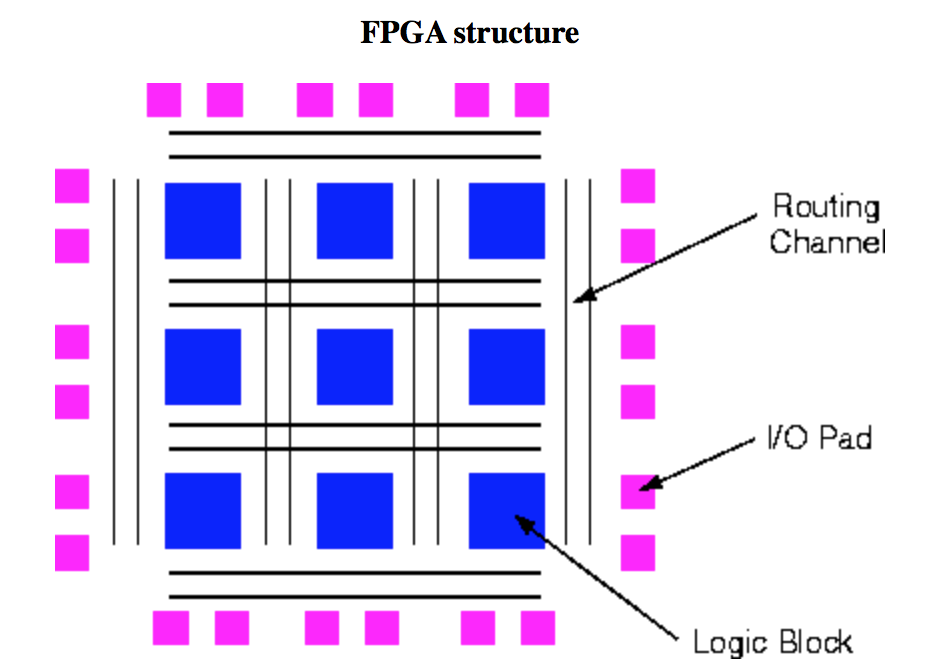
\includegraphics[width=0.7\textwidth]{fpgastructure}
	\caption{Scheme of FPGA components \citep{FPGA_toronto}.}
	\label{fig:fpgastructure}
\end{figure}

\begin{figure}[htbp]
	\centering
	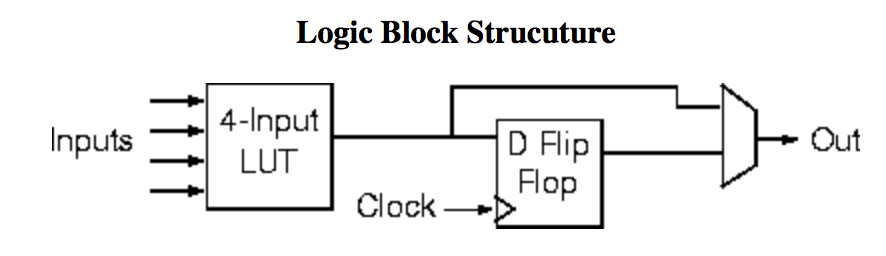
\includegraphics[width=0.7\textwidth]{logicblockstruct}
	\caption{Structure of a logic block \citep{FPGA_toronto}.}
	\label{fig:logicblockstruct}
\end{figure}


The biggest advantage of the \gls{fpga} is that it is able to make multiple processes at the same time by isolating some logic blocks and \gls{io} for a specific task, which is not possible with a \gls{cpu}. A \gls{cpu} needs to run tasks in sequence, one after the other. If different tasks need to be done in a restricted timing, this timing parameter can be crucial. 
By using parallelism and having fast \gls{io}, the \gls{fpga} can be very powerful \citep {FPGA_youtube} \citep{FPGA_center} \citep{FPGA_toronto}. \\

The \gls{fpga} can be programmed using a hardware description language like VHDL or Verilog \citep {FPGA_youtube} \citep{FPGA_center} \citep{FPGA_toronto}. \\

\gls{fpga}'s are more efficient than \gls{cpu}'s but they are also more expensive especially if the purpose is to clone a pre-existing \gls{cpu} without any personal added value. They are also power demanding. The \gls{fpga} has a configuration flash memory which means that there is no need for the user to intervene after a reboot, but at each boot the \gls{fpga} is programmed from scratch using the data from the flash memory. This can drastically increase the boot time as well as the power consumption. It is more complicated to program a \gls{fpga} than using an \gls{cpu} because it has to be designed by the user \citep {FPGA_youtube} \citep{FPGA_center} \citep{FPGA_toronto}. \\








